\documentclass[8pt]{article}

\usepackage[T1]{fontenc}
\usepackage[utf8]{inputenc}
\usepackage[english]{babel}
\usepackage{mathpazo}
\usepackage[scaled]{helvet}
\usepackage{microtype}
\usepackage[letterpaper,margin=1in]{geometry}
\usepackage{amsmath}
\usepackage{amssymb}
\usepackage{booktabs}
\usepackage{array}
\usepackage{enumitem}
\usepackage{float}
\usepackage{tikz}
\usetikzlibrary{arrows.meta,positioning}
\usepackage{xurl}
\usepackage{hyperref}

\hypersetup{
  pdftitle={Volt: Financial Semantics for Option Portfolio Graphs},
  pdfauthor={research@strategynet.ai},
  colorlinks=true,
  linkcolor=blue!50!black,
  citecolor=blue!50!black,
  urlcolor=blue!60!black
}

\setlength{\parindent}{0pt}
\setlength{\parskip}{0.55em}
\setlist{nosep}

\newcommand{\VOLT}{\textsf{Volt}}
\newcommand{\COG}{\texttt{COG}}
\newcommand{\R}{\mathbb{R}}
\newcommand{\Z}{\mathbb{Z}}
\newcolumntype{P}[1]{>{\raggedright\arraybackslash}p{#1}}

\title{\VOLT{}: Financial Semantics for Option Portfolio Graphs}
\author{research@strategynet.ai}
\date{July 2026}

\begin{document}
\maketitle

\begin{abstract}
An option portfolio appears in several operational forms: listed contracts and quantities, an expiration payoff, live exercise and assignment state, executions and cash movements, and model features.  Independent implementations of these forms can disagree about which position was evaluated or traded.  \VOLT{} defines the listed contracts and signed positions as the authoritative portfolio and derives payoff, runtime, compiler, and graph views from that object.  European, Bermudan, and American exercise share one exercise-opportunity representation; the runtime records exercise, assignment, expiry, cash, and delivered underlying as state transitions.  A deterministic graph connects each option position to its portfolio, underlying, and expiry while retaining hashes of the contract portfolio and expiration-payoff projection.  The \COG{} compiler resolves bounded semantic actions to listed contracts and emits aligned action nodes and legal masks.  This paper defines those financial semantics, identifies the equivalence represented by each derived view, and states the implemented boundary supplied to portfolio discovery and sequential control.
\end{abstract}

\section{Introduction}

The security master identifies the listed contract, the position service
records quantity, the risk system attaches marks and sensitivities, the payoff
tool projects expiration cash flows, and the execution ledger records fills.
A research pipeline produces another representation when it converts the
position into model features and outcomes.

A terminal payoff groups portfolios by expiration geometry.  A runtime state
records rights, obligations, cash, inventory, and lifecycle events.  A graph
exposes relationships to a learning model.  An execution journal explains how
the account reached its current state.  Each view retains the identity needed
for its purpose and a link to the contract portfolio.

\VOLT{} begins with listed option contracts and signed quantities.  Contract
terms remain fixed, market observations are timestamped context, and
lifecycle events change an explicit portfolio state.  Terminal payoff and
machine-learning graphs are derived views tied back to the contract portfolio
by versioned content hashes.  The statistical model therefore receives a
stable representation while pricing, execution, exercise, assignment, and
settlement remain governed by declared financial components.

The design supports two research problems.  Portfolio discovery evaluates and
ranks entry portfolios constructed from listed contracts.  Portfolio control
chooses actions repeatedly as the market and account state change.  Both
consume the same contract, runtime, compiler, and graph semantics.

Research on financial contract languages established that a compact contract
description can support several interpretations, including valuation,
evolution, and executable lowering \cite{arnold1995,peytonjones2000}.  Later
work added verified analyses and compilation to parallel payoff evaluation
\cite{bahr2015,annenkov2018}.  Production and standards efforts have applied
related ideas to derivative payouts and lifecycle events
\cite{frankau2009,actus,cdm}.  \VOLT{} applies this separation of meaning and
interpretation to listed-option portfolio search.

\section{Contracts, positions, and market state}
\label{sec:portfolio}

\subsection{Listed contracts}

At decision time \(t\), let
\[
  \mathcal U_t=\{o_1,\ldots,o_d\}
\]
be the eligible listed contracts.  Contract \(o_i\) contains
\[
  o_i=(\mathrm{id}_i,u_i,c_i,r_i,K_i,T_i,m_i,
       \mathcal E_i,\zeta_i),
\]
where \(\mathrm{id}\) is the contract identifier, \(u\) the underlying, \(c\)
the settlement currency, \(r\) the call or put right, \(K\) the strike, \(T\)
the expiry, \(m\) the multiplier, \(\mathcal E\) the exercise-opportunity set,
and \(\zeta\) the settlement rule.

A portfolio is a sparse quantity assignment
\[
  q=(q_1,\ldots,q_d)\in\Z^d.
\]
Positive quantities are long and negative quantities are short.  Repeated
trades in one contract are netted into one \(q_i\).  The fills and fees remain
in the execution journal even when the current quantity becomes zero.

Market observations form a separate state \(c_t\).  Spot, option marks, bid
and ask prices, volatility coordinates, rates, dividends, and liquidity
measurements can change without changing contract identity.  This separation
also determines the unit of a learning example: a portfolio \(q\) observed in
market state \(c_t\).

\subsection{Admissible portfolios}

The position algebra admits every integer quantity vector.  Trading and
research constraints define
\[
  \mathcal C_t
  =\{q\in\mathcal Q^d:g_j(q,c_t,a_t)\leq0,\ j=1,\ldots,J\},
\]
where \(\mathcal Q\) is a bounded quantity set and \(a_t\) is account state.
The functions \(g_j\) may impose leg-count, gross-quantity, liquidity,
exposure, capital, and margin limits.

\VOLT{} implements contract validity, exercise authority, bounded quantity
grammar, point-in-time contract resolution, and several portfolio guards.
Account capital, portfolio margin, and broker eligibility remain inputs from
the application that owns the account.

\section{Derived identities}
\label{sec:identity}

The system retains four identities under four equivalence relations.

\begin{center}
\begin{tabular}{@{}P{0.23\linewidth}P{0.31\linewidth}P{0.37\linewidth}@{}}
\toprule
Identity & Equal when & Information retained \\
\midrule
Contract portfolio &
The net quantity of every listed contract agrees &
Contract terms, exercise style, settlement, multiplier, and quantity \\
Expiration payoff &
The selected-horizon payoff functions agree &
Cash, underlying exposure, and payoff changes at strike knots \\
Runtime state &
The versioned positions, lifecycle, cash, inventory, and sequence agree &
Open rights and obligations plus completed state transitions \\
Graph sample &
The derived node, edge, context, and source hashes agree &
Model features and their links to contract and payoff identities \\
\bottomrule
\end{tabular}
\end{center}

\subsection{Expiration-payoff projection}

For vanilla options on one underlying and expiration, a static European
portfolio can be written
\[
  \Pi(S_T)
  =a+bS_T+\sum_{j=1}^{n}c_j(S_T-K_j)^+,
  \qquad K_1<\cdots<K_n.
\]
Here \(a\) is cash, \(b\) is underlying exposure, and \(c_j\) is the change in
payoff slope at strike \(K_j\).  The identity
\[
  (K-S)^+=K-S+(S-K)^+
\]
converts puts into the same hinge representation.

Let \(\Phi_T(q)\) denote this expiration-payoff projection.  The relation
\[
  q_1\sim_T q_2
  \quad\Longleftrightarrow\quad
  \Phi_T(q_1)=\Phi_T(q_2)
\]
groups contract portfolios that share the selected terminal geometry.
American exercise, assignment, liquidity, funding, transaction costs, and the
path of option marks can distinguish members of one payoff class.  The
contract-portfolio hash is therefore retained alongside the payoff hash.

\subsection{Execution identity}

Position netting and payoff projection operate on the current holding.  The
execution journal records the route into that holding.  If \(a\) is a trade
and \(\mathcal C_t(a)\) its cash consequence, then
\[
  a+(-a)=0
\]
in the position algebra, while a round trip across bid \(b_t\) and ask \(a_t\)
with multiplier \(m\), quantity \(q\), and fees \(f\) produces
\[
  -|q|m(a_t-b_t)-f.
\]
Execution paths reaching the same portfolio may also differ through partial
fills, package execution, legging risk, market impact, financing, or hedge
turnover.  Portfolio comparison can use netted positions without discarding
that evidence.

\section{Exercise and lifecycle semantics}
\label{sec:lifecycle}

\subsection{Exercise opportunities}

Let
\[
  \mathcal T=\{\tau_0,\tau_1,\ldots,\tau_H\}
\]
be the event or observation grid.  Each option declares an exercise set
\(\mathcal E_i\):
\[
\begin{aligned}
  \text{European:}\quad&
    \mathcal E_i=\{T_i\},\\
  \text{Bermudan:}\quad&
    \mathcal E_i=\{t_1,\ldots,t_n=T_i\},\\
  \text{American:}\quad&
    \mathcal E_i=\{\tau_j\in\mathcal T:
      t_{\mathrm{first},i}\leq\tau_j\leq T_i\}.
\end{aligned}
\]
European and Bermudan contracts are restrictions of the American opportunity
representation.  A simulation grid discretizes the American interval; its
spacing and event alignment are experiment assumptions.

Exercise authority belongs to a long holder while the opportunity is open.
Assignment is an external event for a short writer.  The action type and
runtime validation preserve this distinction, preventing a policy from
treating assignment as a voluntary short-side action.

\subsection{State transitions}

Runtime state at event time \(t\) is
\[
  x_t=(x_t^{C},x_t^{P},x_t^{M},x_t^{A},x_t^{R}),
\]
with contract, portfolio, market, account, and protocol components.  One
action and one market observation produce
\[
  (x_{t+1},e_{t+1})
  =F_{\omega}(x_t,a_t,z_{t+1}),
\]
where \(\omega\) identifies the execution and lifecycle rules and
\(e_{t+1}\) contains typed cash, underlying, and consumed-right emissions.

For \(n>0\) physically settled long calls with multiplier \(m\), exercise
emits
\[
  \Delta Q_u=nm,\qquad \Delta C=-nmK.
\]
A long put emits
\[
  \Delta Q_u=-nm,\qquad \Delta C=nmK.
\]
Assignment of a short position reverses the postings.  Cash settlement emits
signed intrinsic value and leaves underlying inventory unchanged.

For example, assignment of one short, physically settled \(100\)-strike put
with multiplier \(100\) consumes the short option, posts \(100\) shares, and
debits \(10{,}000\) units of cash.  The next state carries the shares and cash
into subsequent risk and management decisions.

\subsection{Replay}

Each accepted transition records the schema version, sequence, prior and next
state hashes, action, observation, typed emissions, rule identifier, and
journal-entry hash.  Content hashes use a versioned namespace and canonical
serialization:
\[
  H=\operatorname{SHA256}(
    \text{schema namespace}\Vert0\mathrm{x}00
    \Vert\text{canonical content}).
\]
Replaying the same versioned contract definitions, initial state,
observations, and actions reproduces the state and emission sequence.

\section{Portfolio graph}
\label{sec:graph}

\subsection{Implemented graph schema}

The implemented portfolio graph contains a portfolio node, one underlying
node, one expiry node, and one node for each nonzero option position:
\[
  V=\{v_{\mathrm{portfolio}},v_{\mathrm{underlying}},
       v_{\mathrm{expiry}}\}\cup V_{\mathrm{position}}.
\]
Each position has three typed directed edges:
\[
\begin{aligned}
  v_i&\xrightarrow{\mathrm{position\ in}}v_{\mathrm{portfolio}},\\
  v_i&\xrightarrow{\mathrm{written\ on}}v_{\mathrm{underlying}},\\
  v_i&\xrightarrow{\mathrm{expires\ at}}v_{\mathrm{expiry}}.
\end{aligned}
\]

The position node carries contract identifier, option right, settlement,
exercise style, strike, mark, signed quantity, multiplier, first exercise
time, and exercise-opportunity count.  The underlying node carries spot and
currency; the expiry node carries expiry and time to expiry.  Marks are graph
context; contract terms retain fixed legal and economic definitions.

\begin{figure}[H]
  \centering
  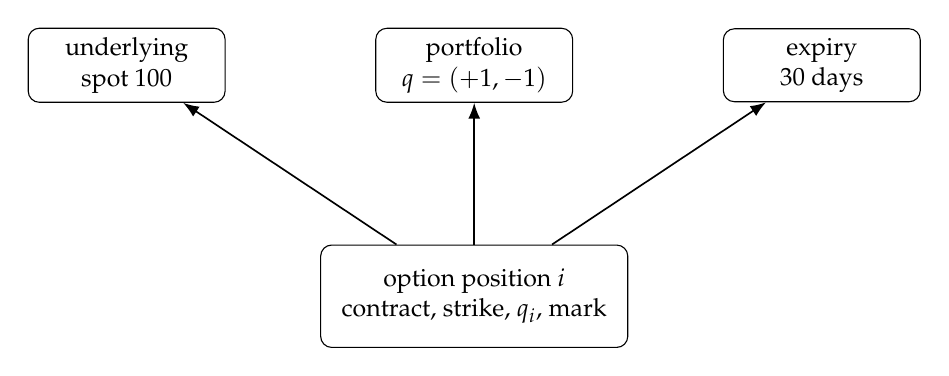
\begin{tikzpicture}[
    node distance=18mm and 19mm,
    every node/.style={font=\small,align=center},
    context/.style={draw,rounded corners,minimum width=25mm,minimum height=9mm},
    position/.style={draw,rounded corners,minimum width=39mm,minimum height=13mm},
    relation/.style={-{Latex[length=2mm]},semithick}
  ]
    \node[context] (underlying)
      {underlying\\spot \(100\)};
    \node[context,right=of underlying] (portfolio)
      {portfolio\\\(q=(+1,-1)\)};
    \node[context,right=of portfolio] (expiry)
      {expiry\\30 days};
    \node[position,below=of portfolio] (position)
      {option position \(i\)\\contract, strike, \(q_i\), mark};

    \draw[relation] (position) -- (underlying);
    \draw[relation] (position) -- (portfolio);
    \draw[relation] (position) -- (expiry);
  \end{tikzpicture}
  \caption{Each nonzero leg creates one option-position node connected to its
  portfolio, underlying, and expiry through the typed relations defined
  above.  The two-position example instantiates the node for the long \(90\)
  call and the short \(110\) call.  Contract quantities determine the
  candidate; spot and marks belong to the decision state.}
  \label{fig:portfolio-graph}
\end{figure}

Figure~\ref{fig:portfolio-graph} contains one candidate--state pair.  Changing
a contract or quantity produces another candidate.  Changing spot, marks, or
valuation time produces another state.  Reordering the position nodes
preserves the graph and portfolio identity.

\subsection{Runtime state/action graph}

The additive \texttt{RuntimeStateActionGraphSample} represents continuing
control states.  It creates one expiry node for each distinct contract expiry
and retains live, exercised, assigned, expired, and closed position nodes.
Cash ledgers, delivered-underlying inventory, and an account node carry the
balances and limits seen by the policy.  Compiler action slots enter as nodes
with their exact contract, quantity, mark, expiry, source rule, and rejection
reason.

The runtime graph adds portfolio-to-account, cash-to-account,
inventory-to-account, action-to-portfolio, action-to-position, and
action-to-account relations.  Position and action nodes connect to their
corresponding underlying and expiry nodes.  One graph can therefore contain
several expiries while preserving exact contract identity.

The exported legal mask first applies compiler guards and contract rules, then
checks declared account limits for live position count, gross option
quantity, minimum cash, absolute underlying inventory, and deterministic
option costs.  These limits provide a reproducible research account model.
Broker portfolio margin, locate rules, and market liquidity remain separate
authorities.

\subsection{Graph identity and targets}

\texttt{PortfolioGraphSample} stores the graph schema version, a feature
sample identifier, the contract-portfolio hash, the expiration-payoff hash,
nodes, edges, and an optional target.  The target is excluded from feature
identity, allowing an evaluator correction to update a label without changing
the candidate--state identifier.

Targets may contain path-aggregated P\&L, drawdown, costs, exercise effects,
or other declared outcomes.  The scenario evaluator produces those values;
the graph transports the structural inputs and provenance to a set model,
graph neural network, optimizer, or analysis tool.

The static graph retains one underlying and one common expiry for
candidate-ranking compatibility.  The runtime graph supplies multi-expiry,
account, inventory, and action nodes.  Multi-underlying, risk-factor, and
event nodes remain extensions.  Each additional relation is measured against
an order-invariant set model through prediction and ranking
\cite{deepsets,relational}.

\section{Compiler and candidate actions}
\label{sec:compiler}

The \COG{} compiler converts versioned structured source into an immutable
financial program:
\[
  \text{source}
  \longrightarrow
  \text{validated contracts and rules}
  \longrightarrow
  \text{compiled artifact}.
\]
Source contains the listed universe, initial positions, candidate grammar,
typed guards, priorities, and an optional scenario objective.  Compilation
validates the schema and contracts, collects source-addressed diagnostics,
normalizes rules, resolves semantic contract coordinates, and records source
and artifact hashes.

At a decision state, the compiled artifact evaluates its guards and emits
stable candidate-action slots with rejection reasons and an aligned legal
mask.  Implemented actions are \texttt{AddLeg}, \texttt{RemoveLeg},
\texttt{ResizeLeg}, \texttt{Wait}, and holder-authorized
\texttt{Exercise}.  A semantic addition can use option right, tenor, and
moneyness or supplied delta coordinates; the point-in-time resolver returns
matching listed contracts in stable order.

The state/action graph combines:
\[
  (\text{portfolio graph},\text{runtime context},
    \text{action nodes},\text{action edges},\text{legal mask}).
\]
Action edges identify the current portfolio, a targeted live position, or the
underlying used by a proposed addition.  A learned policy scores these action
nodes after deterministic contract and lifecycle legality have been applied.
The application composes liquidity, capital, margin, and broker constraints
with the compiler mask.

Multi-leg strategy macros, close and roll plans, account policy, and tensor
lowering remain development work.  Direct portfolio discovery can proceed
with generated signed contract quantities before those conveniences are
available.

\section{Scenario evaluation and evidence}
\label{sec:evaluation}

One scenario path supplies timestamped underlying observations, option marks
or quotes, and external events.  \texttt{ScenarioSimulator} opens the
portfolio, applies the declared fill and cost rules, advances lifecycle
actions through the runtime, and records pathwise and terminal P\&L with leg
attribution.

Two implemented fill conventions establish an explicit execution boundary.
\texttt{DeclaredMark} uses the supplied mark as a synthetic fill.
\texttt{CrossAtTouch} buys at the ask and sells at the bid, and requires the
corresponding quote side.  Historical or generated research must additionally
declare the mark source, missing-data rule, assignment model, management
policy, and option-valuation method used between observations.

For path cohort \(\Xi_t=\{\xi_1,\ldots,\xi_M\}\), the evaluator produces
\[
  y_t(q)
  =A\left(
    \{R(q,\xi_m;c_t,\nu,\mu,\alpha,\omega)\}_{m=1}^{M}
  \right).
\]
Here \(\nu\) is the mark or valuation rule, \(\mu\) the management and exercise
rule, \(\alpha\) the assignment rule, \(\omega\) the execution and settlement
rules, and \(A\) the outcome aggregation.  These versioned inputs give the
graph target its financial interpretation.

Decision-time features use observations available at \(t\).  Future
observations on \(\Xi_t\) create outcomes.  Dataset records therefore retain
event time, as-of time, source revision, visible contract universe, quote
rule, exercise and assignment assumptions, and split membership.

\section{Implemented boundary}
\label{sec:implementation}

\begin{center}
\begin{tabular}{@{}P{0.27\linewidth}P{0.62\linewidth}@{}}
\toprule
Component & Current public implementation \\
\midrule
Contracts &
\texttt{OptionContract}, European/Bermudan/American exercise schedules,
cash or physical settlement, and \texttt{Position} \\
Market evidence &
Versioned source manifests, historical or generated observation provenance,
ordered option observations, and declared proxy or top-of-book authority \\
Portfolio identities &
\texttt{CanonicalPortfolio}, netted quantities, semantic hashes, and
\texttt{TerminalPayoffProjection} \\
Lifecycle &
\texttt{CogRuntime}, immutable \texttt{PortfolioState}, exercise,
assignment, expiry, cash and underlying emissions, and journals \\
Scenarios &
\texttt{ScenarioSimulator}, declared-mark and touch fills, fees, pathwise
P\&L, terminal P\&L, leg attribution, and result hashes \\
Candidates and compiler &
\texttt{CandidateGrammar}, \texttt{CogCompiler}, guarded rules, compiled
artifacts, action sets, rejection reasons, and legal masks \\
Graph views &
\texttt{PortfolioGraphSample}, \texttt{CompiledPortfolioGraphSample}, and
\texttt{StateActionGraphSample}; \texttt{graph\_export} converts declared
marked contracts and quantity vectors into canonical graph samples \\
\bottomrule
\end{tabular}
\end{center}

The repository also contains deterministic \texttt{cog}, \texttt{graph},
\texttt{zap}, and \texttt{risk} examples.  They exercise compilation,
candidate enumeration, graph export, portfolio reduction, and an educational
risk display using synthetic data.  A research driver uses the public graph
exporter with generated American CRR marks, fixed exercise and assignment
policies, constrained portfolio enumeration, path-labelled targets, and a
Deep Sets baseline.  A parameter-matched typed graph network consumes the
exported nodes and position-to-portfolio, position-to-underlying, and
position-to-expiry relations.  Its market adapters, trained weights, and
experiment records remain outside the public financial-semantics crate.

Executable historical quote adapters, account and margin policy, promotion of
the research hedge-policy interface, richer account and action relations,
strategy macros, and GPU lowering remain integration work.

\section{Validation}

Semantic tests compare direct portfolio payoff with the hinge projection,
check that position order leaves portfolio and graph identities unchanged,
and replay lifecycle journals from versioned inputs.  Compiler tests check
diagnostic collection, rule priority, stable branch order, aligned action
masks, and state binding.

The first learning study adds three empirical checks.  First, every target is
recomputed by the financial evaluator from its recorded assumptions.  Second,
chronological splits keep label-horizon observations out of model inputs.
Third, the typed graph network receives the same contracts, market context,
targets, candidate split, and optimization budget as the Deep Sets baseline.
The current fixed-expiry topology establishes the executable comparison;
edge and relation ablations measure richer graph structure next.

These tests separate three sources of failure: financial semantics, dataset
construction, and statistical estimation.  A model result can be traced to
the candidate--state graph, the exact contract portfolio, the path cohort,
and the runtime evidence that produced its outcome.

\section{Conclusion}

Listed contracts and signed quantities determine the portfolio exported to a
learning system.  Exercise schedules and runtime transitions determine its
continuing state, while fills and journals record changes in cash, option
rights, and underlying inventory.  The payoff projection and graph are
derived records linked by versioned identifiers to those inputs and
transitions.

The implemented graph contains portfolio, underlying, expiry, and
option-position nodes with typed edges.  The \COG{} compiler adds
point-in-time action nodes and deterministic legal masks.  Path evaluation
supplies supervised outcomes.  These records support the direct portfolio
search developed in the discovery paper and the state/action interface used
by sequential control.

\begin{thebibliography}{9}

\bibitem{arnold1995}
B. R. T. Arnold, A. van Deursen, and M. Res,
\emph{An Algebraic Specification of a Language for Describing Financial
Products},
ICSE-17 Workshop on Formal Methods Application in Software Engineering,
pp.~6--13, 1995.

\bibitem{peytonjones2000}
S. Peyton Jones, J.-M. Eber, and J. Seward,
\emph{Composing Contracts: An Adventure in Financial Engineering},
ICFP, 2000.

\bibitem{bahr2015}
P. Bahr, J. Berthold, and M. Elsman,
\emph{Certified Symbolic Management of Financial Multi-party Contracts},
ICFP, pp.~315--327, 2015,
\url{https://doi.org/10.1145/2784731.2784747}.

\bibitem{annenkov2018}
D. Annenkov and M. Elsman,
\emph{Certified Compilation of Financial Contracts},
PPDP, 2018,
\url{https://doi.org/10.1145/3236950.3236955}.

\bibitem{frankau2009}
S. Frankau, D. Spinellis, N. Nassuphis, and C. Burgard,
\emph{Commercial Uses: Going Functional on Exotic Trades},
Journal of Functional Programming, 19(1), pp.~27--45, 2009,
\url{https://doi.org/10.1017/S0956796808007016}.

\bibitem{actus}
ACTUS Financial Research Foundation,
\emph{Algorithmic Contract Types Unified Standards: Fundamentals},
\url{https://www.actusfrf.org/methodology}.

\bibitem{cdm}
FINOS,
\emph{Common Domain Model: Event Model},
\url{https://cdm.finos.org/docs/event-model/}.

\bibitem{deepsets}
M. Zaheer, S. Kottur, S. Ravanbakhsh, B. Póczos, R. Salakhutdinov, and
A. Smola,
\emph{Deep Sets},
Advances in Neural Information Processing Systems, 2017,
\url{https://arxiv.org/abs/1703.06114}.

\bibitem{relational}
P. W. Battaglia et al.,
\emph{Relational Inductive Biases, Deep Learning, and Graph Networks},
2018,
\url{https://arxiv.org/abs/1806.01261}.

\end{thebibliography}

\end{document}
